  
  If we expand the probabilities given further more by substituting the value of x and only considering 0 to 4 hours as the probability of studying in the remaining hours is zero, we get
  
  \begin{table}[ht]
  
 \centering
  
  \begin{tabular}{|c|c|c|c|c|c|}
    \hline
    x &  0 & 1 & 2 & 3 & 4\\
    \hline
    $\Pr\brak{X=x}$ & 0.1& k& 2k & 2k & k\\
    \hline
    
\end{tabular}
\caption{Given probabilities}
\label{Table_1}
\end{table}
we also know that,
\begin{align}
    \sum_{k = 0}^4 \Pr\brak{X = k} = 1 \label{eq 2.0.1}
\end{align}

By substituting the probabilities in \eqref{eq 2.0.1}
\begin{align}
& \implies 0.1 + k + 2k + 2k + k = 1 \\
& \implies 6k = 0.9 \label{eq 2.0.3}
\end{align}

Therefore, from \eqref{eq 2.0.3}
\begin{align}
    k = 0.15
\end{align}
  
 So from \ref{Table_1}
  \begin{table}[ht]
  
  \centering
  \begin{tabular}{|c|c|c|c|c|c|}
    \hline
    x &  0 & 1 & 2 & 3 & 4\\
    \hline
    $\Pr\brak{X=x}$ & 0.1& 0.15& 0.3 & 0.3 & 0.15\\
    \hline
    
\end{tabular} 
\caption{Probabilities after finding k}
\end{table}

\begin{figure}[ht]
    \centering
    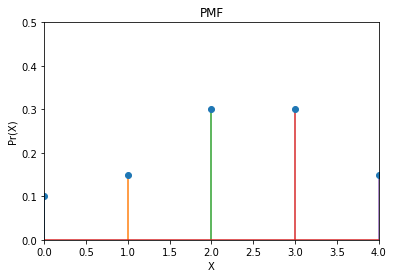
\includegraphics[width=\columnwidth]{solutions/5/28/Figures/PMF.png}
    \caption{Probability Mass Function (PMF)}
    \label{Figure_1}
\end{figure}

We know that, Cumulative Distributive Function (CDF) 
\begin{align}
    F(x) = \Pr\brak{X \le x}
\end{align}

\begin{table}[ht]
  
  \centering
  \begin{tabular}{|c|c|c|c|c|c|}
    \hline
    x &  0 & 1 & 2 & 3 & 4\\
    \hline
    $F(X)$ & 0.1& 0.25& 0.55 & 0.85 & 1\\
    \hline
    
\end{tabular} 
\caption{CDF}
\label{Table_2}
\end{table}

\begin{figure}[ht]
    \centering
    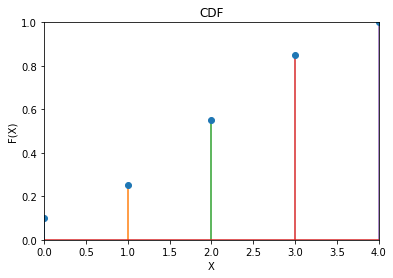
\includegraphics[width=\columnwidth]{solutions/5/28/Figures/CDF.png}
    \caption{Cumulative Distributive Function (CDF)}
    \label{Figure_2}
\end{figure}

And also, 
\begin{align}
     \Pr\brak{x < X \le y} = F\brak{y} - F\brak{x} \label{eq 2.0.6}
\end{align}
         \begin{enumerate}
        \item Probability of studying at least two hours 
           \begin{align}
            & \implies \sum_{k = 2}^4 \Pr\brak{X = k} = \Pr\brak{X \ge 2}\\
            & \implies \Pr\brak{1 < X \le 4} 
        \end{align}
        From \eqref{eq 2.0.6} and \eqref{Table_2}
        \begin{align}
            & = F(4) - F(1)\\
            & = 1 - 0.25\\
            & = 0.75
        \end{align}
        
        \item Probability of studying exactly two hours
        \begin{align}
            & = \Pr\brak{X = 2}\\
            & = 0.3
        \end{align}
        
        \item Probability of studying at most two hours 
        \begin{align}
          & \implies \sum_{k = 0}^2  \Pr\brak{X = k} = \Pr \brak{X \le 2}
         \end{align}
        From \eqref{Table_2}
        \begin{align}
            & = F(2)\\
            & = 0.55
        \end{align}
    \end{enumerate}
  
    \begin{table}[ht]
   
    \centering
  \begin{tabular}{|c|c|c|}
    \hline
    $\Pr\brak{X \geq 2}$ &  $\Pr \brak{X = 2}$ & $\Pr\brak{X \leq 2}$\\
    \hline
     0.75& 0.3& 0.55 \\
    \hline
    Case 1 &Case 2 &Case 3\\
    \hline
\end{tabular} 
 \caption{Final solution}
 \label{Table_3}
\end{table}

\begin{figure}[ht]
    \centering
    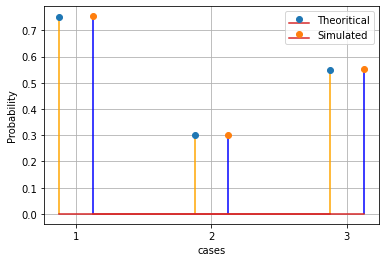
\includegraphics[width=\columnwidth]{solutions/5/28/Figures/stem.png}
    \caption{Simulation and Theoretical Comparison}
    \label{Figure_3}
\end{figure}

